\documentclass[onecolumn]{article}
%\usepackage{url}
%\usepackage{algorithmic}
\usepackage[a4paper]{geometry}
\usepackage{datetime}
\usepackage[margin=2em, font=small,labelfont=it]{caption}
\usepackage{graphicx}
\usepackage{mathpazo} % use palatino
\usepackage[scaled]{helvet} % helvetica
\usepackage{microtype}
\usepackage{amsmath}
\usepackage{subfigure}
% Letterspacing macros
\newcommand{\spacecaps}[1]{\textls[200]{\MakeUppercase{#1}}}
\newcommand{\spacesc}[1]{\textls[50]{\textsc{\MakeLowercase{#1}}}}

\title{\spacecaps{Assignment Report 1: Process and Thread Implementation}\\ \normalsize \spacesc{CENG2034, Operating Systems} }

\author{Osman Batuhan Şahin\\osmanbatuhansahin@posta.mu.edu.tr\\https://github.com/osmanbatuhansahin}
%\date{\today\\\currenttime}
\date{\today}

\begin{document}
\maketitle

\begin{abstract}
In this assignment, one of our goal is learning how to use python os, requests, threading and platform libraries. Learning operating system basics, remember phyton and linux skills and how threads works is another goals. I assume using threads while getting url status codes will make our job faster before assignment. It happened.
\end{abstract}


\section{Introduction}
This assignment is important because I practice and learned how operating systems works, specially linux. I used python and linux for this assignment.

\section{Assignments}
At fourth question, I could not write urls in threads. Then I write urls in an array and give indexes to threads. Printing 5 minute loadavg value is not possible with one line code like os.getloadavg(). I also print it with using an arrays first index.



\section{Results}


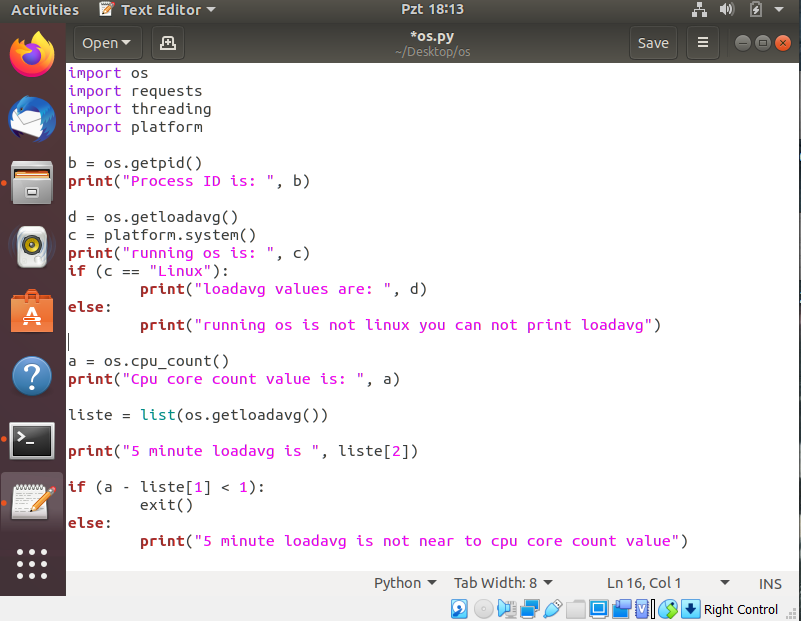
\includegraphics[width=\textwidth]{cozum123.PNG}
Code of Question 1-2-3





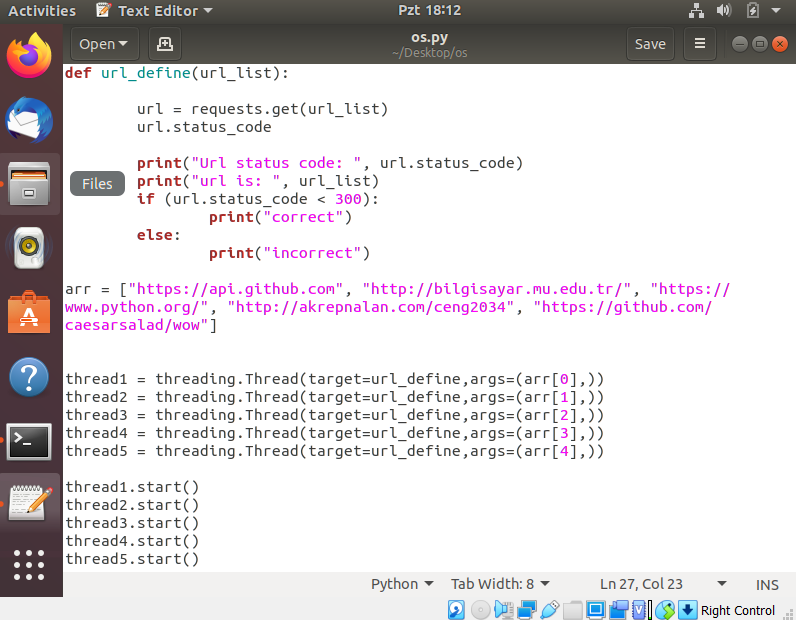
\includegraphics[width=\textwidth]{cozum4.PNG}
Code of Question 4



\section{Conclusion}
Every computer scientist should know operation system basics. It will make our softwares more efficiently.


\nocite{*}
\bibliographystyle{plain}
\bibliography{references}
\end{document}